
%%%%%%%%%%%%%%%%%%%%%%%%%%%%%%%%%%%%%%%%%%%%%%%%%%%%%%%%%%%%%%%%%%%%%%%%%
%           Capítulo 3: NOMBRE                   %
%%%%%%%%%%%%%%%%%%%%%%%%%%%%%%%%%%%%%%%%%%%%%%%%%%%%%%%%%%%%%%%%%%%%%%%%%

\chapter{Diseño e implementación}

En el presente capítulo se retoman los conceptos desarrollados en el capítulo anterior para describir el diseño e implementación del sistema transmisor láser que utiliza la tarjeta de desarrollo STM32F446RE como generador de pulsos e interfaz de usuario, el amplificador operacional OPA350 cómo elemento principal del driver de corriente basado en el diseño de la fuente de corriente Howland y finalmente se expone la operación y funcionamiento del diodo láser de 1550 nm como una fuente de pulsos ópticos modulados.El diagrama del sistema antes mencionado es ilustrado en la Figura \ref{Diagrama_tx} y es descrito a detalle en las secciones siguientes. 

\begin{figure}[H]
    \centering
    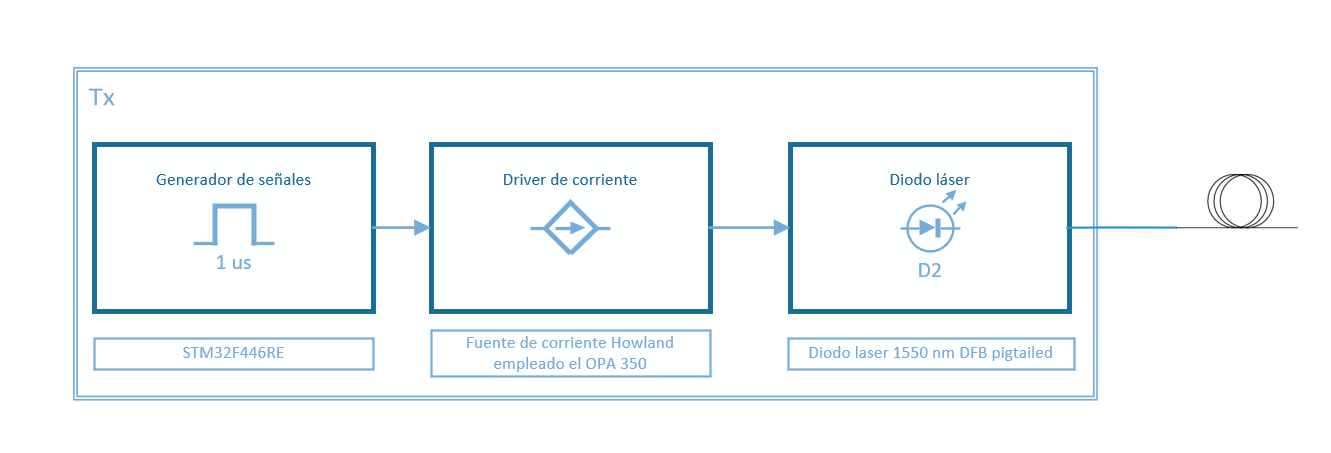
\includegraphics[width=14cm]{Figures/diagrama_1_pieces.png}
    \caption{Diagrama del sistema transmisor láser pulsado}
    \label{Diagrama_tx}
\end{figure}

\section{Tarjeta de desarrollo STM32}

La tarjeta de desarrollo STM32F446RE (STM32 Nucleo-64) pertenece a una familia de tarjetas de desarrollo con diferentes configuraciones y prestaciones; contienen embebido un microcontrolador STM32 con un empaquetado LQFP64\footnote{Siglas en ingles de Low-profile Quad Flat Package 64 Terminals (\textit{Encapsulado Cuadrado Plano de Perfil Bajo de 64 terminales})} 

El microcontrolador STM32 embebido en la tarjeta de desarrollo STM32F446RE tiene un núcleo Arm\footnote{Anteriormente ARM por las siglas en inglés de Advanced RISC MAchine y actualmente Arm por Acorn RISC Machine} Cortex-M4 basado en la  arquitectura RISC (Reduced Instruction Set Computer) de 32 bits y una Unidad de Punto Flotante(FPU por las siglas en inglés de \textit{Floating-Point Unit}). 












% \chapter{Diseño del experimento}
% En este capítulo, se presenta la introducción al desarrollo de la tesis, ya sea el modelo matemático o las bases del proyecto, etc.
% Ejemplo de cita  [\citet{latex}]
% Ejemplo de cita [\citeauthor{RR73}]
 % The \cite command functions as follows:
 %   \citet{key} ==>>                Jones et al. (1990)
 %   \citet*{key} ==>>               Jones, Baker, and Smith (1990)
 %   \citep{key} ==>>                (Jones et al., 1990)
 %   \citep*{key} ==>>               (Jones, Baker, and Smith, 1990)
 %   \citep[chap. 2]{key} ==>>       (Jones et al., 1990, chap. 2)
 %   \citep[e.g.][]{key} ==>>        (e.g. Jones et al., 1990)
 %   \citep[e.g.][p. 32]{key} ==>>   (e.g. Jones et al., p. 32)
 %   \citeauthor{key} ==>>           Jones et al.
 %   \citeauthor*{key} ==>>          Jones, Baker, and Smith
 %   \citeyear{key} ==>>             1990





%%%%%%%%%%%%%%%%%%%%%%%%%%%%%%%%%%%%%%%%%%%%%%%%%%%%%%%%%%%%%%%%%%%%%%%%%
%                          Descripción de la planta                     %
%%%%%%%%%%%%%%%%%%%%%%%%%%%%%%%%%%%%%%%%%%%%%%%%%%%%%%%%%%%%%%%%%%%%%%%%%
% \section{Sección}
% El sistema blah, blah. Ejemplo de cita \citep{texbook}
% La figura (\ref{planta})                     %hace referencia a la imagen "planta" el número se inserta automáticamente
%  ilustra los componentes de la planta.

% \begin{figure}
%   \centering
%     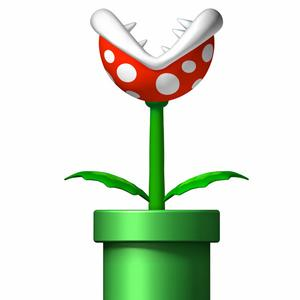
\includegraphics[scale=0.5]{Capitulo3/figs/planta.jpg}      %Ruta completa de la imagen, porque se compila desde el archivo tesis.tex
%   \caption{Descripción de la planta}            %Pie de imagen
%   \label{planta}                            %nombre de referencia
% \end{figure}




% %%%%%%%%%%%%%%%%%%%%%%%%%%%%%%%%%%%%%%%%%%%%%%%%%%%%%%%%%%%%%%%%%%%%%%%%%
% %                          Modelado                                     %
% %%%%%%%%%%%%%%%%%%%%%%%%%%%%%%%%%%%%%%%%%%%%%%%%%%%%%%%%%%%%%%%%%%%%%%%%%
% \section{\textcolor{Azul}{Sección en color azul}}
% \subsection{Subsección}
% Antes de comenzar, se definen  en la tabla ~\ref{tab:tabla} los parámetros y variables utilizadas

% %%%%%%%%Tabla Nombres de parámetros
% \begin{table}[ht]                             %Inicia el entorno table debajo del texto
% \centering\                                     %   centra la tabla
% \begin{tabular}{||c | c ||}                     %inicia entorno tabular con doble línea en las orillas, 2 columnas con el contenido centrado (c)
% \hline                                          %inserta línea horizontal
% \hline
% Nombre Parámetro/Variable & Símbolo\\
% \hline
% \hline
% Masa del péndulo & $m$ \\
% \hline
% Masa del carro & $M$\\
% \hline
% Distancia del eje de giro al centro de masa & $l$ \\
% \hline
% Aceleración gravitatoria & $g$ \\
% \hline
% Momento de inercia péndulo respecto del eje de giro& $J$ \\
% \hline
% Ángulo del péndulo respecto del eje vertical & $\theta$\\
% \hline
% Velocidad angular del péndulo & $\dot{\theta}$, $\omega$\\
% \hline
% Distancia del carro respecto al centro del riel & x\\
% \hline
% Velocidad del carro & $\dot{x}$, $v$\\
% \hline
% \hline
% \end{tabular}
% \caption[Parámetros dinámicos del carro-péndulo]{\textbf{Parámetros dinámicos del carro-péndulo} - Estos son los valores de parámetros utilizados en el diseño y las simulaciones, corresponden a los valores reales.}
% \label{tab:tabla}                              %etiqueta para referencia
% \end{table}

% \blindtext


% %%%%%%%%%%%%%%%%%%%%%%%%%%%%%%%%%%%%%%%%%%%%%%%%%%%%%%%%%%%%%%%%%%%%%%%%%
% %                          Subsección
% %%%%%%%%%%%%%%%%%%%%%%%%%%%%%%%%%%%%%%%%%%%%%%%%%%%%%%%%%%%%%%%%%%%%%%%%%

% \subsection{Otra subsección}

% \Blindtext